\section{Master Theorem}
Normalmente, dato un problema con size $n$ lo dividiamo in asottoproblemi con dimensione $n/b$ ed $f(n)$ costo della "combina" di entrambe le cose.
Otteniamo come ricorrenza (con $a \geq 1, b > 1$):
\begin{equation*}
    T(n) = aT(n/b) + f(n)
\end{equation*}
Esso stabilisce che, avendo a che fare con le ricorrenze di questo tipo, avremmo tre casi:
\begin{itemize}
    \item Se il costo della risoluzione dei sotto-problemi ad ogni livello aumenta di un certo fattore, il valore di $f(n)$ diventerà polinomialmente più piccolo di $n^{\log_b}a$. Pertanto, la complessità temporale è oppressa dal costo dell'ultimo livello, vale a dire $n^{\log_b}a$.
    \begin{equation*}
        f(n) = O(n^{\log_b a-\epsilon}) \quad (\epsilon > 0)
    \end{equation*}
    \item Se il costo per risolvere il sotto-problema ad ogni livello è quasi uguale, allora il valore di $f(n)$ sarà $n^{\log_b}a$. Pertanto, la complessità temporale sarà $f(n)$ volte il numero totale di livelli $n^{\log_b}a * log(n)$.
    \begin{equation*}
        f(n) = \Theta(n^{\log_b a}) \Rightarrow T(n) = \Theta(n^{\log_b a} \cdot \log n)
    \end{equation*}
    \item Se il costo della risoluzione dei sottoproblemi ad ogni livello diminuisce di un certo fattore, il valore di $f(n)$ diventerà polinomialmente più grande di $n^{\log_b}a$. Pertanto, la complessità temporale è oppressa dal costo di $f(n)$.
    \begin{equation*}
        \begin{rcases}
            f(n) = \Omega(n^{\log_b a+\epsilon}) \quad (\epsilon > 0) \\
            \exists \; 0 < k < 1 : a \cdot f(n/b) \leq k \cdot f(n)
        \end{rcases}
        \Rightarrow T(n) = \Theta(f(n))
    \end{equation*} 
\end{itemize}

L'idea è che la funzione si ripeta come rapporto ricorsivamente, questo corrisponde alla divisione in due parti e ancora in due parti, ecc.
\begin{equation*}
    T(n) = f(n) + a \cdot T(\frac{n}{b}) = f(n) + af(\frac{n}{b}) + a^2 f(\frac{n}{b^2}) + \ldots + a^{\log_bn} f(\frac{n}{b^{\log_bn}}) = n^{\log_ba}
\end{equation*}

\begin{center}
    \begin{tabular}{c}
        \\ 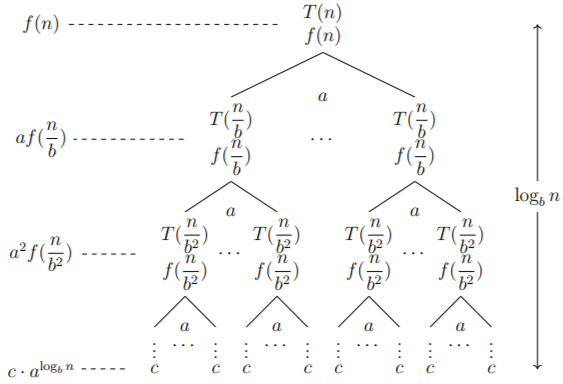
\includegraphics[width=0.7\textwidth]{image/MasterTheorem.png} \\ \\
    \end{tabular}
\end{center}

Confronta tra di loro $f(n)$ e $n^{\log_ba}$:
\begin{itemize}
    \item se vince $f(n) \Rightarrow \Theta(f(n))$
    \item se pareggiano $\Rightarrow \Theta(n^{\log_ba} \cdot \log n)$
    \item se vince $n^{\log_ba} \Rightarrow \Theta(n^{\log_ba})$
\end{itemize}

\newpage